\documentclass{beamer}
\usepackage{beamerthemesplit}
\usepackage{subfig}
\usepackage{amssymb,amsmath,mathtools}
\usepackage{amsfonts,booktabs}
\usepackage{lmodern,textcomp}
\usepackage{color}
\usepackage{tikz}
\usepackage{natbib}
\usepackage{multicol}
\usepackage{ctex}
\usepackage[level]{datetime}
\usepackage{listings}


\usetheme{Warsaw}
\newdateformat{ukdate}{\monthname[\THEMONTH] \ordinaldate{\THEDAY} , \THEYEAR}
\lstset{
 columns=fixed,       
 numbers=left,                                        % 在左侧显示行号
 numberstyle=\tiny\color{gray},                       % 设定行号格式
 frame=none,                                          % 不显示背景边框
 backgroundcolor=\color[RGB]{245,245,244},            % 设定背景颜色
 keywordstyle=\color[RGB]{40,40,255},                 % 设定关键字颜色
 numberstyle=\footnotesize\color{darkgray},           
 commentstyle=\it\color[RGB]{0,96,96},                % 设置代码注释的格式
 stringstyle=\rmfamily\slshape\color[RGB]{128,0,0},   % 设置字符串格式
 showstringspaces=false,                              % 不显示字符串中的空格
 language=c++,                                        % 设置语言
}


\title{基于生成式先验的人像视频编辑}
\author{汪兆辰}
\date{\ukdate\today}

\begin{document}

\begin{frame}
    \titlepage
\end{frame}

\begin{frame}
    \frametitle{用户验证}
    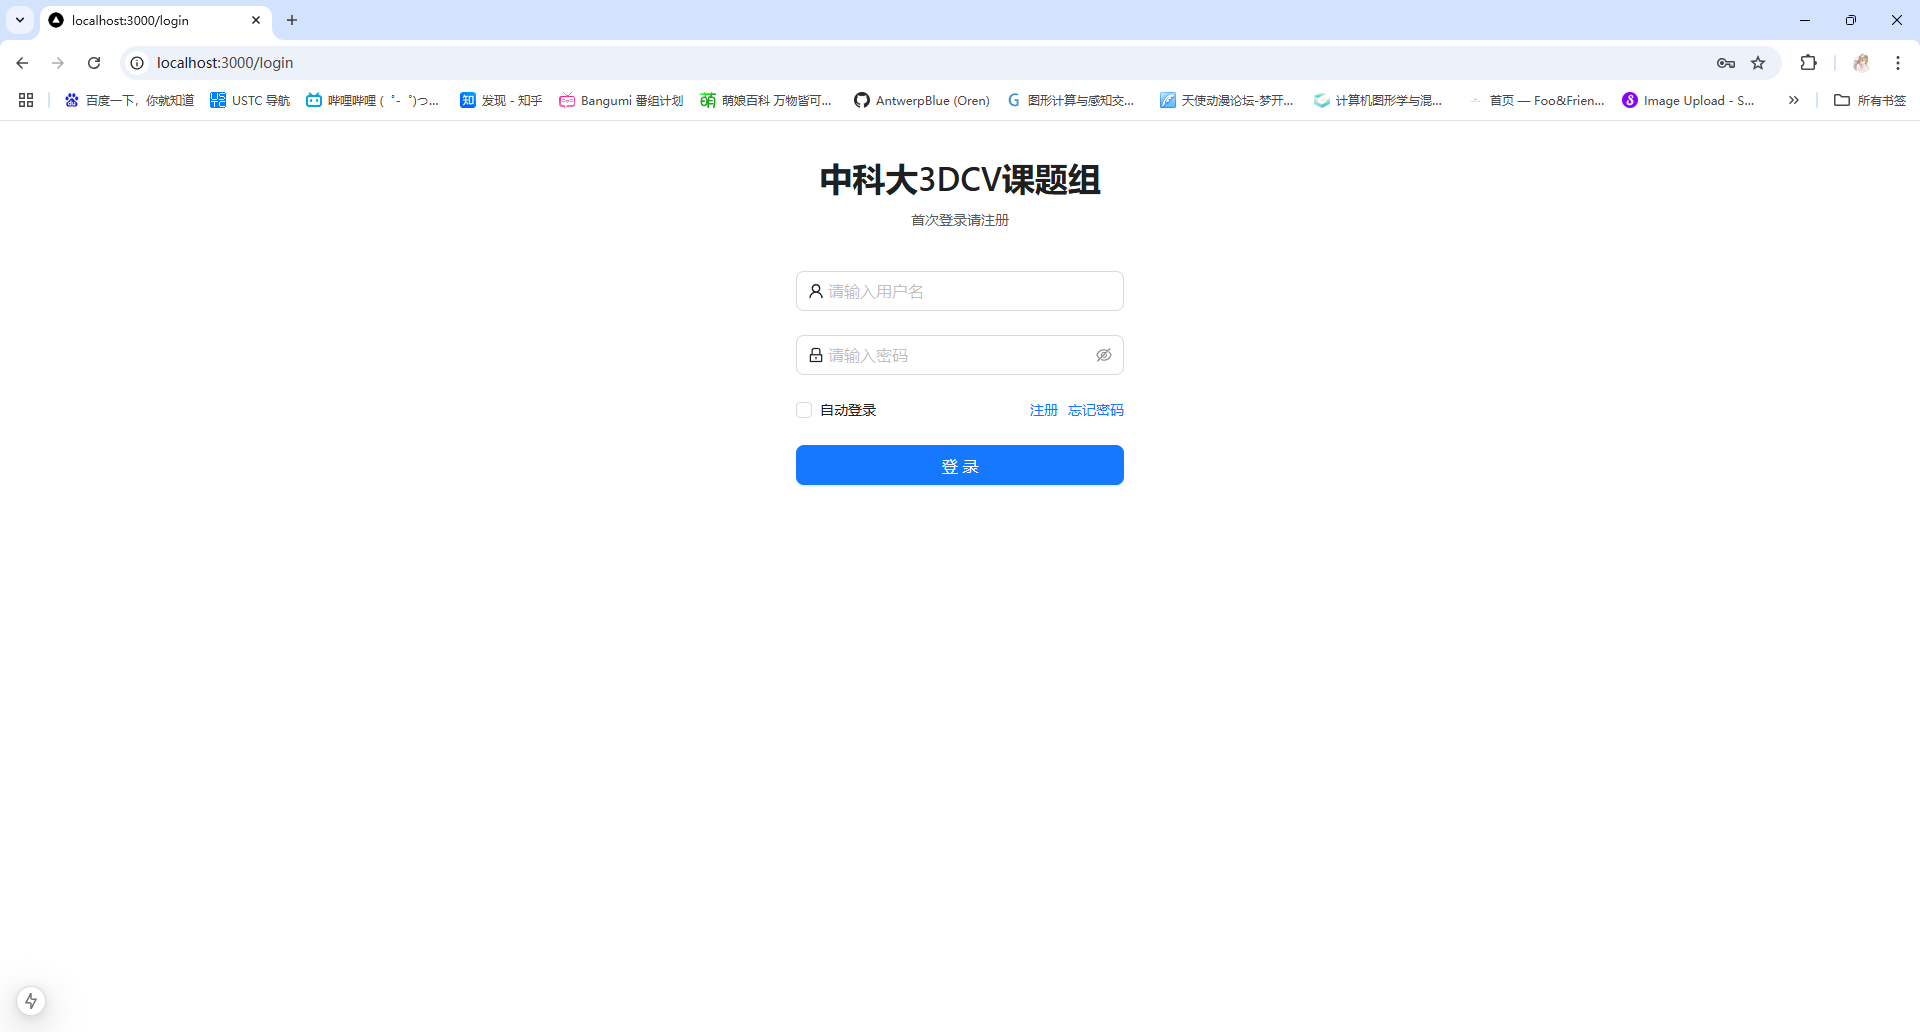
\includegraphics[width=\textwidth]{pic1.png}
\end{frame}

\begin{frame}
    \frametitle{用户验证}
    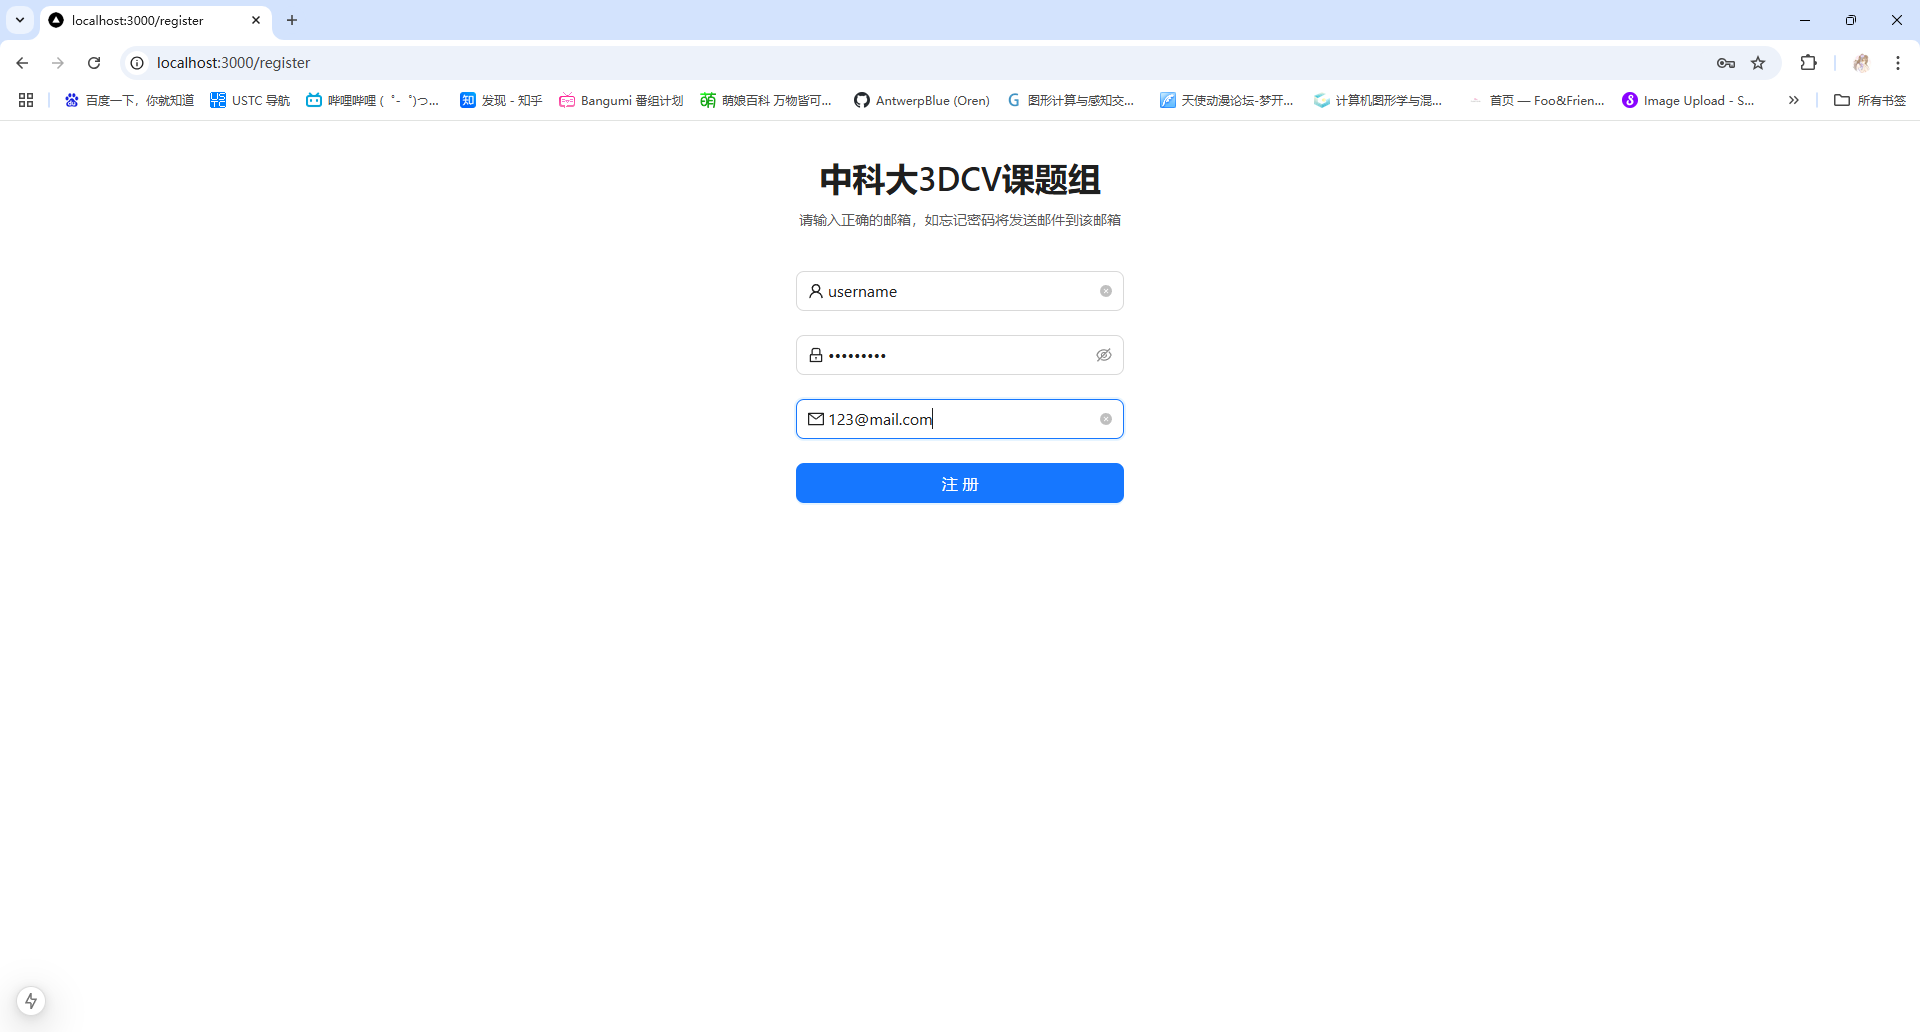
\includegraphics[width=\textwidth]{pic2.png}
\end{frame}

\begin{frame}
    \frametitle{用户验证}
    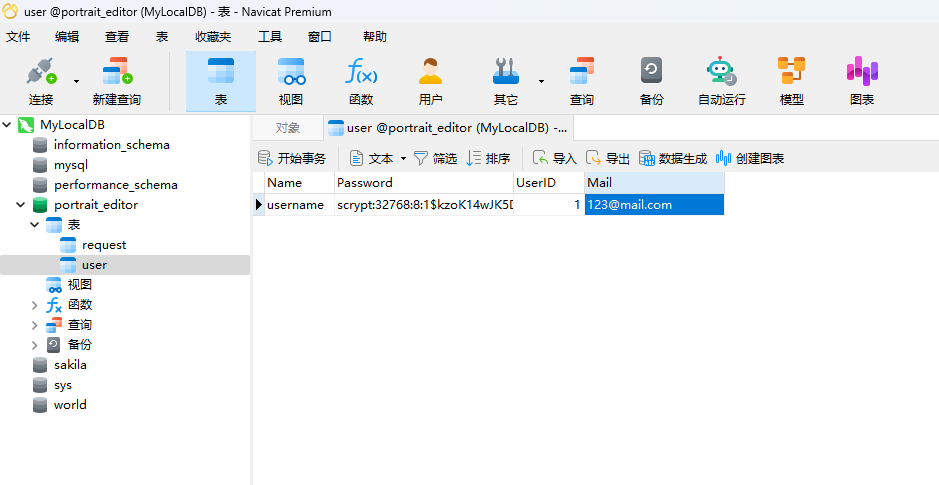
\includegraphics[width=\textwidth]{pic3.png}
\end{frame}

\begin{frame}
    \frametitle{主页面}
    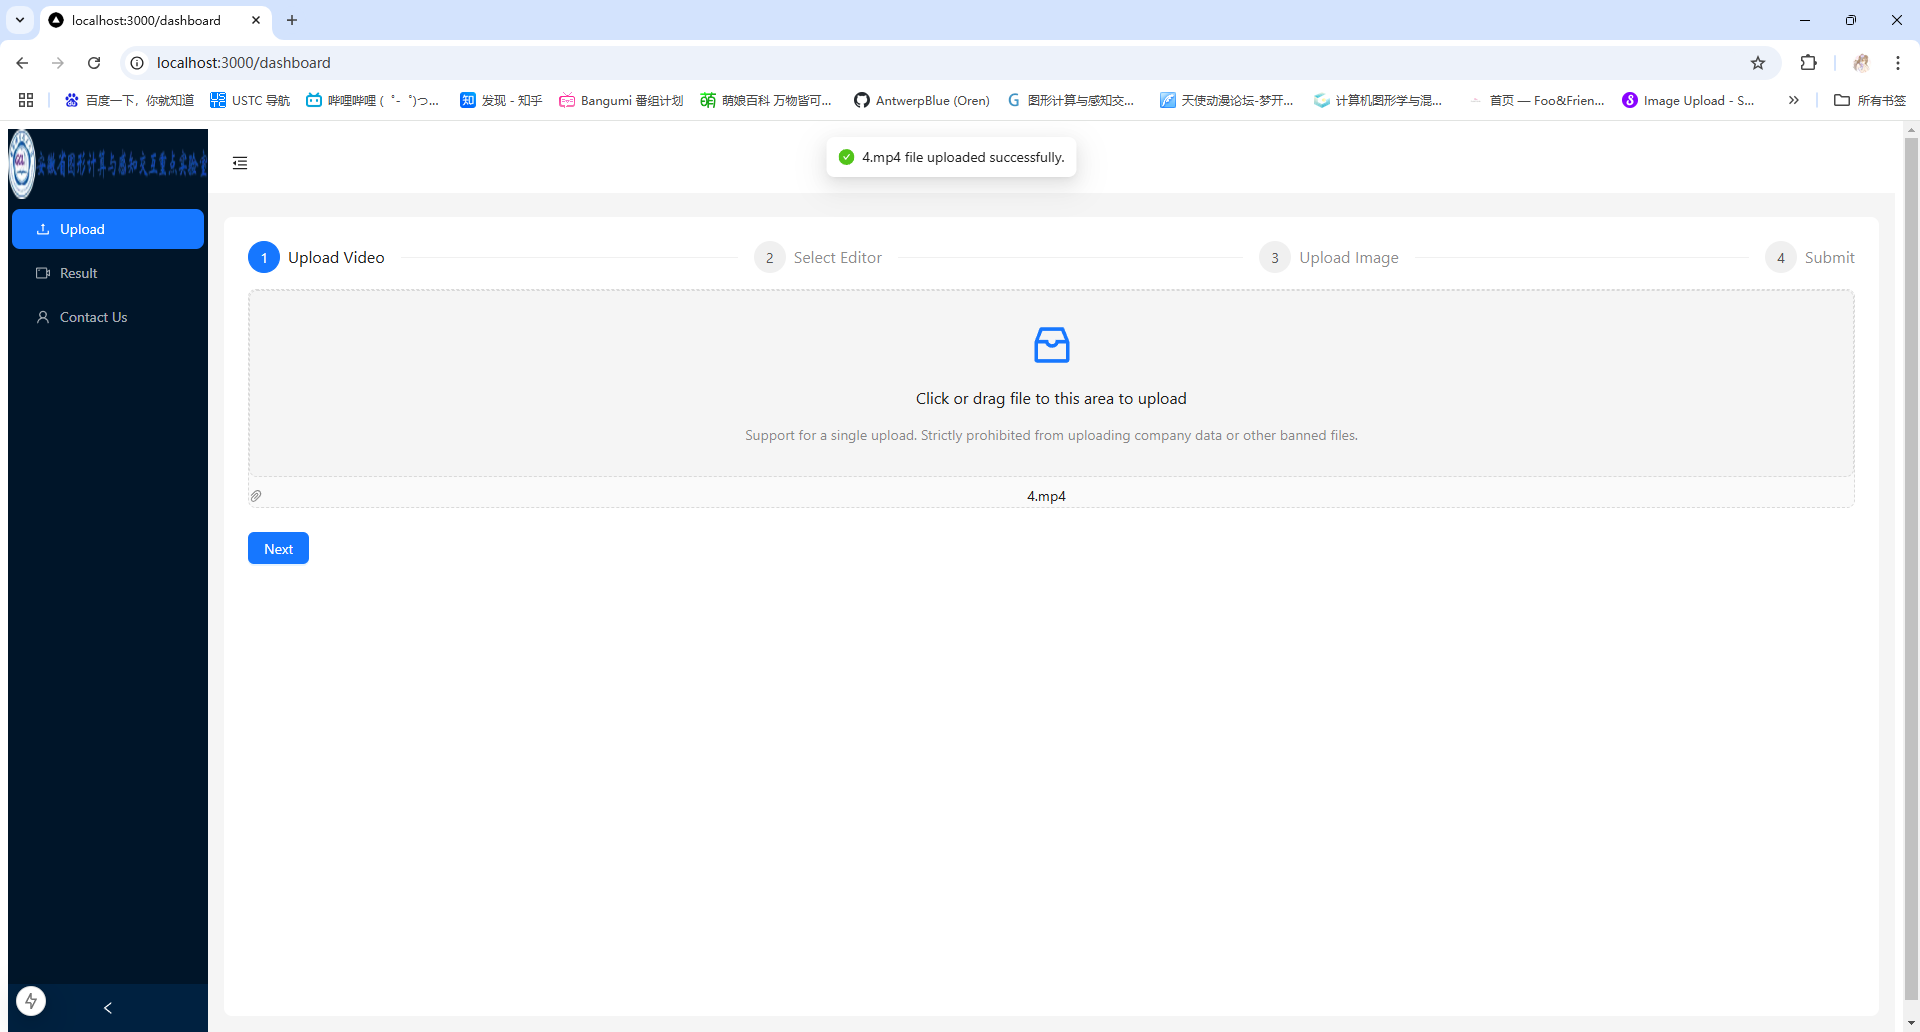
\includegraphics[width=\textwidth]{pic4.png}
\end{frame}

\begin{frame}
    \frametitle{主页面}
    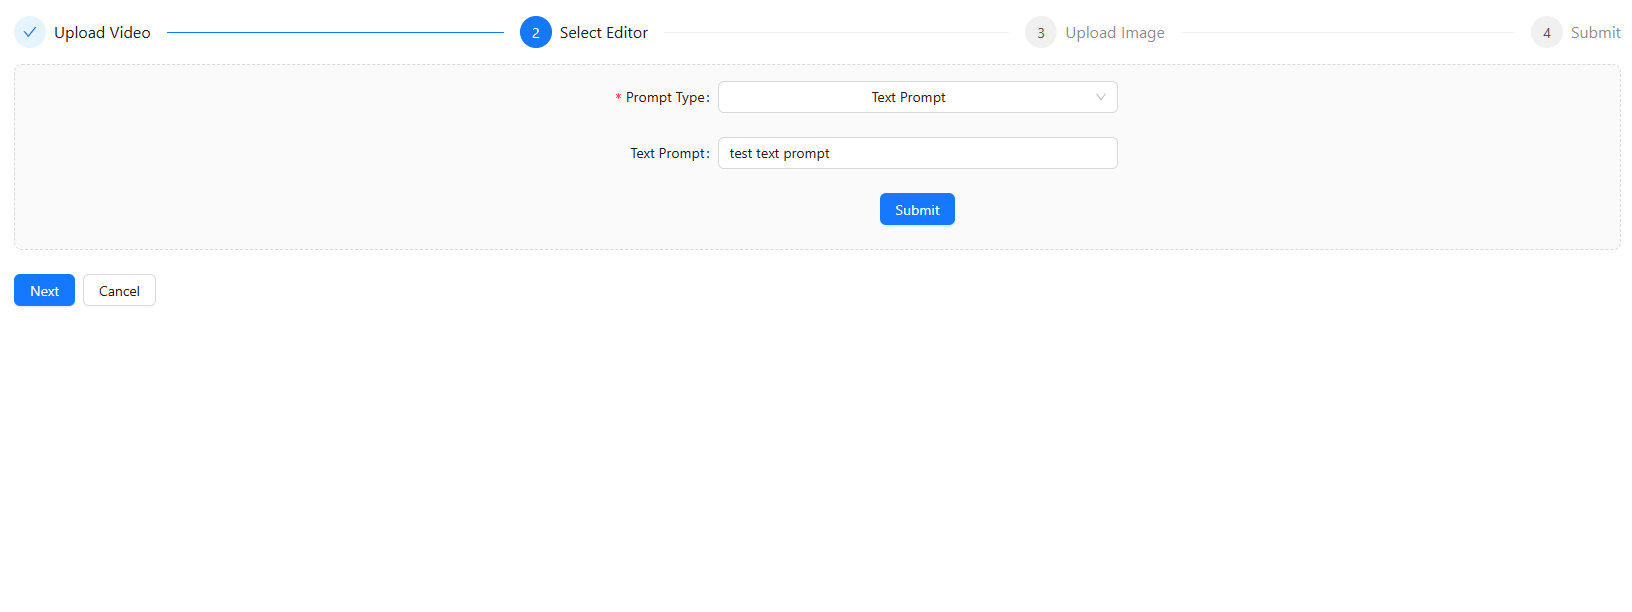
\includegraphics[width=\textwidth]{pic5.png}
\end{frame}
\begin{frame}
    \frametitle{主页面}
    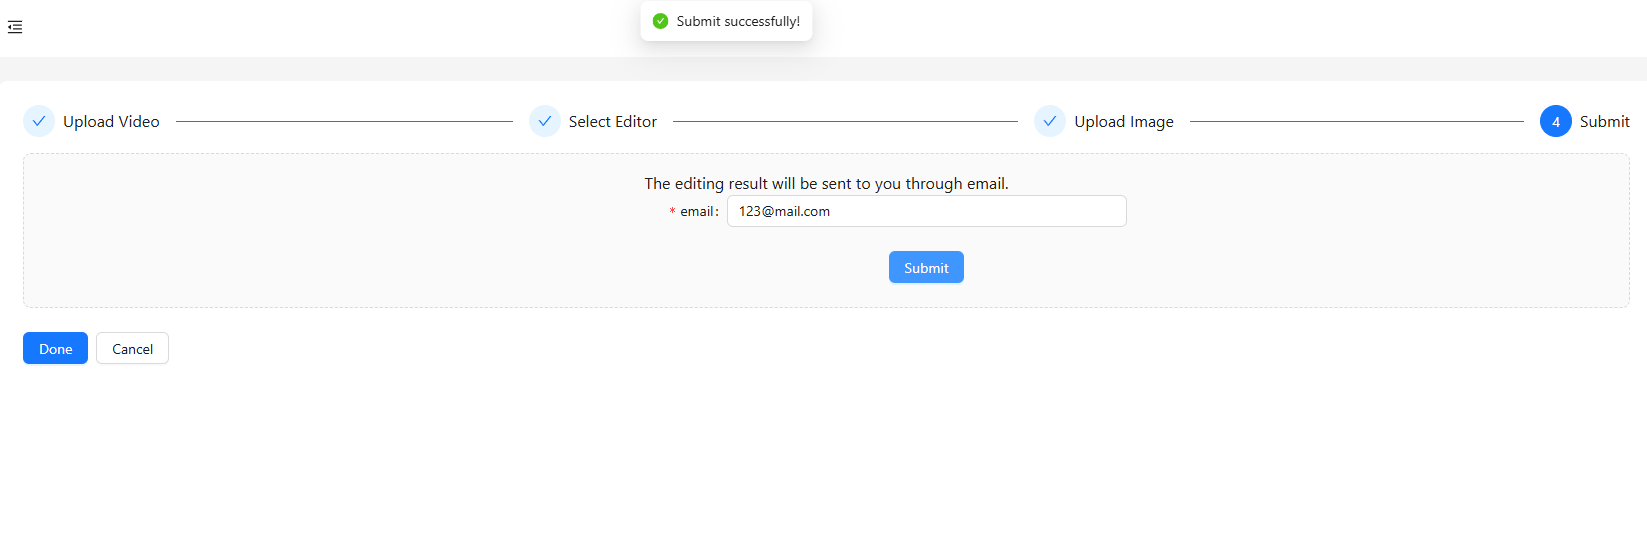
\includegraphics[width=\textwidth]{pic6.png}
\end{frame}
\begin{frame}
    \frametitle{主页面}
    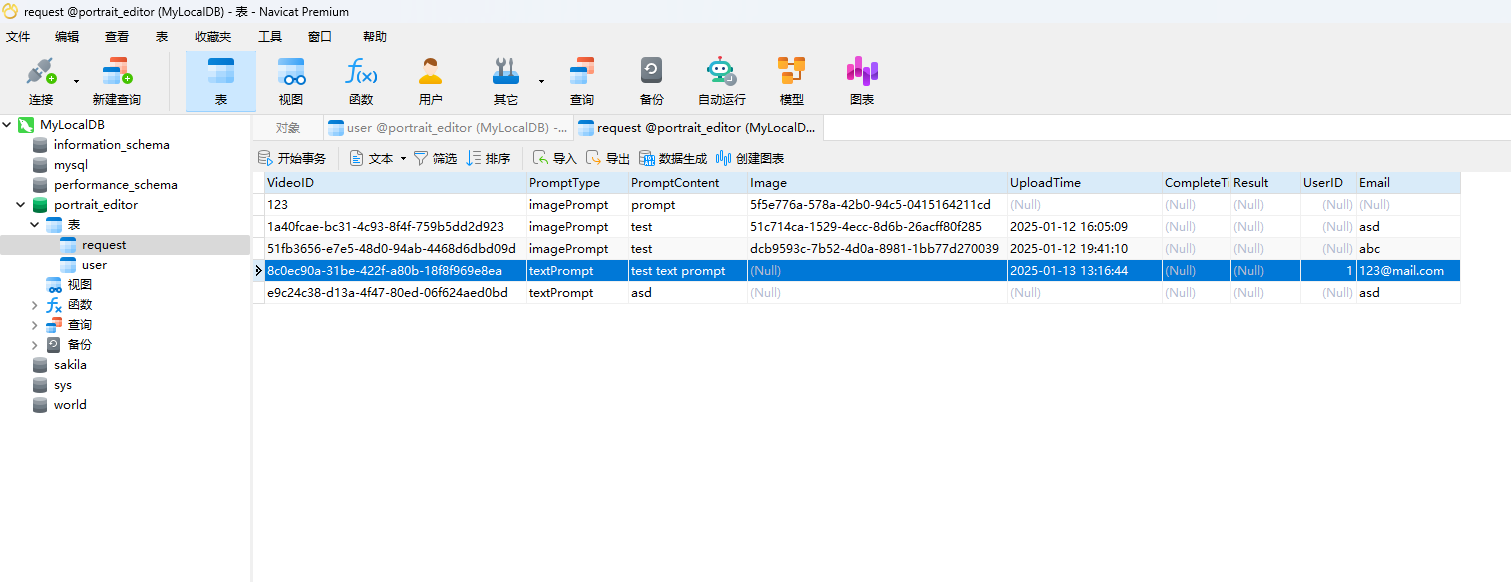
\includegraphics[width=\textwidth]{pic7.png}
\end{frame}

\begin{frame}
    \frametitle{目前进展}
    \begin{itemize}
        \item 客户端的功能已经基本完成,后续需要部署在服务器上
        \item 考虑到后续可能需要将实验室的其他成果整合进来,后续需要实现可以自定义添加新的算法
        \item 为了方便数据的采集与管理,以及使用图形界面添加新算法,考虑在用户分组上添加管理员权限
    \end{itemize}
\end{frame}


\end{document}